\documentclass[11pt]{article}
\usepackage{graphicx}
\usepackage{tcolorbox}
\usepackage{amsmath}
\usepackage{multicol}
\usepackage{amssymb}
\usepackage{amsthm}
\usepackage{amsfonts}
\usepackage{float}
\usepackage[font=small,skip=0pt]{caption}
\usepackage{booktabs}
\makeatletter
\captionsetup[figure]{skip=0pt}
\title{\vspace{-5.0cm}KTH Royal Institute of Technology\\ DD2424-VT19-1 Deep Learning in Data Science\\ Assignment 2}
\author{Marina Herrera Sarrias }
\begin{document}
\maketitle

\begin{tcolorbox}
$i)$ State how you checked your analytic gradient computations and whether you think that your gradient computations were bug free. Give evidence for these conclusions.
\end{tcolorbox}

I verified the analytical computations of the gradients using numerical estimations. The results can be found in the table below.

\begin{table}[H]
	\centering
	\begin{tabular}{llll} 
		\toprule
		& \multicolumn{2}{c}{Maximum Relative Error} &   \\ 
		\cline{2-3}
		& Finite Difference & Centered Difference    &   \\ 
		\cline{2-3}
		$W_{1}$ & 3.62e-03             & 1.96e-03               &   \\
		$b_{1}$ & 8.84e-06          & 8.54e-07               &   \\
		$W_{2}$ & 6.05e-05             & 8.90e-06               &   \\
		$b_{2}$ & 1.01e-04             & 1.15e-07               &   \\
		\bottomrule
	\end{tabular}
\caption{Maximum Relative error between numerical and analytical gradient vectors computations.}
\label{table:1}
\end{table}

We can verify that the centered difference formula provides more accuracy in approximating to the analytical computations of the gradients.

			
\begin{figure}[H]
	\centerline{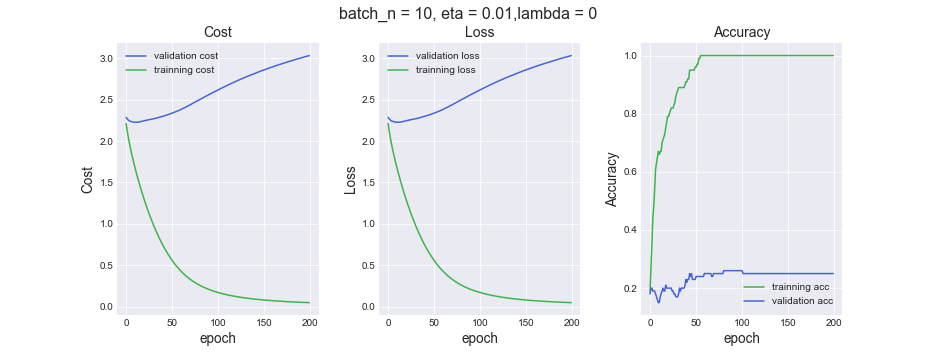
\includegraphics[width=180mm,scale=0.7]{test1.png}}
	\caption{The graph of the training and validation cost, loss and accuracy computed after every epoch. The network was trained with the following parameter settings$:$ \texttt{n\_batch}$=100$ \texttt{eta}$=.01$, \texttt{n\_epochs}$=40$ and  \texttt{lambda}$=1$.}
	\label{fig:1}
\end{figure}

\begin{tcolorbox}
$ii)$The curves for the training and validation loss/cost when using the cyclical learning rates with the default values, that is replicate Figures $3$ and $4$. Also comment on the curves.
\end{tcolorbox}
\begin{figure}[H]
	\centerline{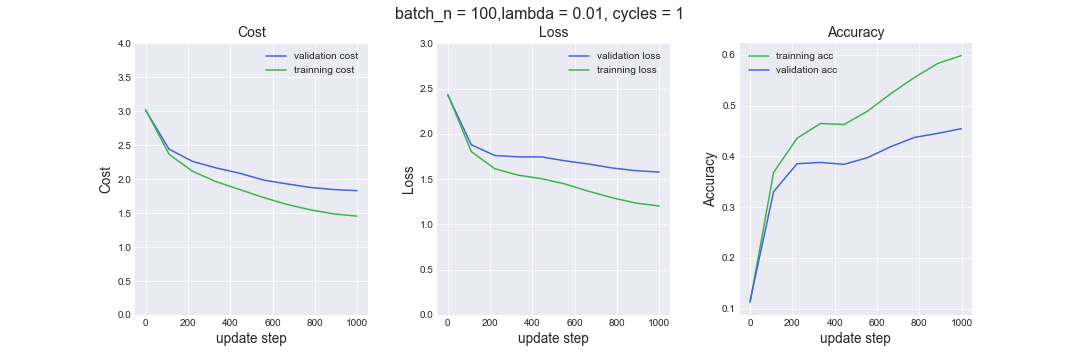
\includegraphics[width=180mm,scale=0.7]{test2.png}}
	\caption{The graph of the training and validation cost, loss and accuracy computed after every epoch. The network was trained with the following parameter settings$:$ \texttt{n\_batch}$=100$ \texttt{eta}$=.01$, \texttt{n\_epochs}$=40$ and  \texttt{lambda}$=1$.}
	\label{fig:2}
\end{figure}
\begin{figure}[H]
	\centerline{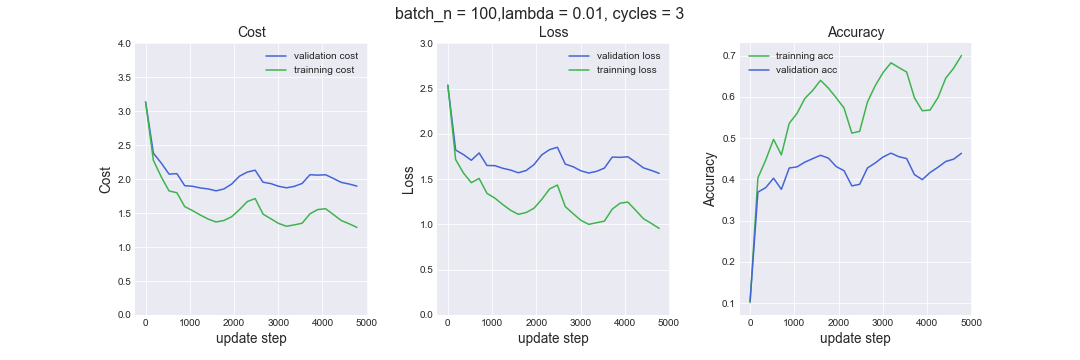
\includegraphics[width=180mm,scale=0.7]{test3.png}}
	\caption{The graph of the training and validation cost, loss and accuracy computed after every epoch. The network was trained with the following parameter settings$:$ \texttt{n\_batch}$=100$ \texttt{eta}$=.01$, \texttt{n\_epochs}$=40$ and  \texttt{lambda}$=1$.}
	\label{fig:3}
\end{figure}
\begin{tcolorbox}
$iii)$ State the range of the values you searched for lambda, the number of cycles used for training during the coarse search and the hyper-parameter settings for the 3 best performing networks you
trained.
\end{tcolorbox}

\begin{tcolorbox}
$iv)$ State the range of the values you searched for lambda, the number of cycles used for training during the ne search, and the hyper-parameter settings for the 3 best performing networks you trained.
\end{tcolorbox}
\begin{tcolorbox}
$v)$ For your best found  \texttt{lambda} setting (according to performance on the validation set),train the network on all the training data (all the batch data), except for $1000$ examples in a validation set, for $3$ cycles. Plot the training and validation loss plots and then report the learnt network's performance on the test data.
\end{tcolorbox}

\end{document}
